\documentclass[conference]{IEEEtran}

\usepackage{amsmath,amssymb,bm}
\usepackage{booktabs}
\usepackage{graphicx}
\usepackage{xcolor}
\usepackage{url}
\usepackage{tikz}
\usetikzlibrary{arrows.meta,positioning}


\title{Activation-Aligned Asynchronous Learned Residual CEM-MPC for Position-Controlled Manipulators}

\author{\IEEEauthorblockN{Anonymous Author(s)}
\IEEEauthorblockA{\textit{Affiliation and contact information omitted for review}}}

\begin{document}
\maketitle

\begin{abstract}
Position-controlled manipulators accept absolute joint references, so a sampling MPC plan can become stale while it is being optimized. We study asynchronous residual CEM-MPC for this setting. A GRU predicts closed-loop actuator-reference dynamics; CEM plans bounded corrections around a continuous IK nominal; and a 100~Hz execution layer reconstructs the current nominal and applies an age-aligned residual packet. On an ABB IRB~2400 MuJoCo model, fixed-delay FullVirtual reduced TCP RMSE by 39.55~mm (58.1\%, 95\% CI 36.87--42.10~mm) relative to NaiveDelayed. Under nominal conditions, ThreadedASAP differed from FullVirtual by 0.054~mm (95\% CI $-1.094$--1.303~mm), reduced RMSE by 10.84~mm relative to Projected Direct IK, and reduced it by 4.21~mm relative to Preview IK. Planner end-to-end latency was 44.92/49.04~ms at p50/p95, above the 10~ms command period; the asynchronous execution layer maintained the reported soft-real-time boundary.
\end{abstract}

\begin{IEEEkeywords}
learned dynamics, model predictive control, cross-entropy method, asynchronous MPC, residual control, robot manipulators
\end{IEEEkeywords}

\section{Introduction and Related Work}
\label{sec:introduction}
Position-controlled robot interfaces accept absolute joint references rather than direct torques. The realized motion can differ from the reference because of joint-servo dynamics, kinematic inaccuracies, structural compliance, transmission effects, saturation, and discrete execution \cite{lee2021nested,lange1994path}. Continuous IK provides a reliable nominal controller, but actuator lag can still produce task-space tracking error.

A learned forward model provides a data-driven alternative when an analytical model of the closed-loop plant is unavailable \cite{hewing2020learning,nagabandi2018neural}. Recurrent models can use histories of state and actuator-reference commands to represent trajectory error dynamics \cite{ma2025trajectory}. In this paper, the model predicts the closed-loop response to absolute actuator references and supplies rollouts to the planner.

The cross-entropy method updates a sampling distribution from elite candidate sequences \cite{deboer2005tutorial}. Learned dynamics, trajectory sampling, and CEM are established ingredients of model-based control \cite{chua2018pets}; GPU-parallel sampling MPC has also been demonstrated for high-rate manipulator control \cite{bhardwaj2022storm}. Residual control retains a nominal controller and optimizes or learns a bounded correction \cite{johannink2019residual}. Here, continuous IK supplies that nominal and CEM searches residual joint-reference corrections. CEM and residual control are not claimed as contributions.

The deployment difficulty is temporal. When learned CEM requires more than the 10~ms command period, the plant continues to evolve during optimization. A plan tied to its launch state and launch-time reference can thus be obsolete when it becomes available. Lowering the replan rate does not correct this state, reference, and history mismatch if old absolute commands are simply cached.

Real-time iteration, computational-delay compensation, advanced-step, and asynchronous MPC address related scheduling problems \cite{diehl2005rti,zavala2009advanced,findeisen2004delay,dirckx2025asap}. Successor-state prediction has also been used to solve a tube-based manipulator MPC problem one step ahead \cite{luo2024smooth}. We build on these ideas rather than claiming to introduce asynchronous MPC. Our focus is their adaptation to history-conditioned learned residual CEM under an absolute position-reference interface: the plan is anchored at its predicted activation state and represented as a timestamped residual packet that is reconciled with the current IK nominal and shared command projection at execution.

Recent manipulator studies include data-driven robust MPC for constrained pose tracking \cite{chen2024ddrmpc}, online incremental-model adaptation with time-delay estimation and recursive least squares \cite{wang2025incremental}, and recurrent trajectory-error prediction \cite{ma2025trajectory}. Constrained sampling-based manipulator MPC increasingly emphasizes projection and physical constraint satisfaction \cite{wang2025constrained}; sampling MPC with fast local feedback has likewise been studied beyond manipulators \cite{belvedere2026feedback}. These works motivate reporting pose tracking, multi-step model error, constraint satisfaction, projection activity, and feedback saturation. In contrast, our scope is a MuJoCo-only study of closed-loop actuator-reference dynamics and activation-time alignment, without online model adaptation, a robust-MPC guarantee, or a physical-robot claim.

This paper makes three contributions, with the first two forming the central method:
\begin{enumerate}
  \item future activation-state and GRU-history alignment for a learned residual CEM planner operating through an absolute position-reference interface;
  \item execution-time reanchoring of timestamped residual packets to the current IK nominal, which prevents an aligned plan from replaying stale absolute commands; and
  \item matched virtual/threaded evaluation quantifying stale-plan degradation, latency recovery, planner--execution discrepancy, packet behavior, projection activity, and soft-real-time execution.
\end{enumerate}
Bounded fast feedback, exact task-space reranking, and two-stage projection are supporting execution mechanisms and measured deployment trade-offs rather than coequal core contributions.

\section{Learned Residual Planner}
\label{sec:planner}

\subsection{Plant, Interface, and Learned Transition}
We consider a six-degree-of-freedom ABB IRB~2400 model simulated in MuJoCo \cite{todorov2012mujoco}, with
\begin{equation}
  \bm{x}_t=[\bm{q}_t^\top,\dot{\bm{q}}_t^\top]^\top\in\mathbb{R}^{12},
  \qquad \bm{u}_t=\bm{q}^{\mathrm{ref}}_t\in\mathbb{R}^{6}.
\end{equation}
The input is the absolute target of the position actuator. MuJoCo advances at 2~ms and the command layer uses five physics substeps, giving $\Delta t=10$~ms. We use the frozen ABB\_IRB2400.xml task-space reference suite and clean commit \texttt{77505a5}; the evidence manifest records the checkpoint, normalizer, reference hashes, and software environment.

The main model is a GRU with aligned history tokens
\begin{equation}
  \bm{z}_i=[\bm{q}_i^\top,\dot{\bm{q}}_i^\top,(\bm{q}^{\mathrm{ref}}_i)^\top]^\top.
\end{equation}
It predicts a velocity increment and reconstructs the next state as
\begin{align}
 \widehat{\Delta\dot{\bm q}}_{t+1}&=f_\theta(\bm z_{t-L+1:t}),\\
 \hat{\dot{\bm q}}_{t+1}&=\dot{\bm q}_t+\widehat{\Delta\dot{\bm q}}_{t+1},\qquad
 \hat{\bm q}_{t+1}=\bm q_t+\hat{\dot{\bm q}}_{t+1}\Delta t.
\end{align}
Training and online rollout use the same aligned $[\bm{x}_t,\bm{u}_t]$ convention. The frozen checkpoint is \texttt{gru\_20260717\_182930}; it uses history length 16 and a 20-step rollout-loss training objective. On 20 new held-out MuJoCo rollouts, its 20-step joint-position RMSE was 0.0216~rad at action standard deviation 0.5 and 0.0441~rad at 0.8; the lower-amplitude group had no divergent rollout. These results show usable short-horizon prediction within the sampled training-action coverage, not stable generalization to arbitrary excitation.

\subsection{IK Nominal and Residual CEM}
A continuous bounded damped-least-squares IK solver maps the desired task-space trajectory to $\bm q^{\mathrm{IK}}$ \cite{wampler1986dls}. For a plan intended to activate at $t_a$, define the joint-range-clipped nominal
\begin{equation}
 \bar{\bm q}^{\mathrm{IK}}_k=
 \operatorname{clip}_{\mathcal Q}(\bm q^{\mathrm{IK}}_{t_a+k+1}).
\end{equation}
The final planner uses a compiled two-stage projection. It screens the full CEM population with a cheap requested-command approximation. A deduplicated exact validation pool then contains the final elites, the best sequence found across the search, the final mean, and the zero-residual baseline. Every pool member is passed through the braking-aware command projector and rolled out again. The 100~Hz execution layer independently applies the same physical projection to every dispatched command.

CEM searches normalized residuals $\bm\rho_k\in[-1,1]^6$,
\begin{equation}
 \bm r_k=\bm\rho_k\odot\bm r_{\max},\qquad
 \tilde{\bm q}^{\mathrm{ref}}_k=
 \operatorname{clip}_{\mathcal Q}(\bar{\bm q}^{\mathrm{IK}}_k+\bm r_k),
 \label{eq:planner-request}
\end{equation}
where $\tilde{\bm q}^{\mathrm{ref}}_k$ is the requested command used by the approximate population rollout. Each CEM iteration includes the zero-residual candidate and current mean.

Let $\alpha_k=\gamma^k/\sum_{j=0}^{H-1}\gamma^j$ denote the normalized temporal discount. The approximate joint-space cost used for population screening is
\begin{align}
 J_{\rm approx}={}&\sum_{k=0}^{H-1}\alpha_k\bigl[
 w_q\ell_q(\hat{\bm q}_{k+1},\bm q^d_k)
 +w_{\dot q}\ell_{\dot q}(\hat{\dot{\bm q}}_{k+1},
 \dot{\bm q}^d_k) \notag\\
 &\quad+w_r\ell_r(\bm r_k)
 +w_s\ell_s(\tilde{\bm q}^{\rm ref}_k,\hat{\bm q}_k)
 \notag\\
 &\quad+w_{\dot r}\ell_{\dot r}(\dot{\bm r}_k)
 +w_{\ddot r}\ell_{\ddot r}(\ddot{\bm r}_k)\bigr]
 \notag\\
 &+w_{\rm first}\ell_{\rm first}
 +w_{\mathcal Q}B_{\mathcal Q}
 +w_{\dot{\mathcal Q}}B_{\dot{\mathcal Q}},
 \label{eq:approx-cost}
\end{align}
where $\dot{\bm r}_k=(\bm r_k-\bm r_{k-1})/\Delta t$ and
$\ddot{\bm r}_k=(\dot{\bm r}_k-\dot{\bm r}_{k-1})/\Delta t$ use the physical control interval. The servo proxy compares action $k$ with its pre-action state $\hat{\bm q}_k$, not $\hat{\bm q}_{k+1}$. Each soft joint-position or velocity barrier is a discounted mean plus a weighted maximum over the horizon and joints. A predicted hard joint-limit violation assigns infinite cost.

The \emph{exact-projection and kinematic final-pool score} additionally uses the exact physical command projector and MuJoCo forward kinematics on learned predicted joint states,
\begin{equation}
 J_{\rm exact}=J_{\rm approx}
 +w_p\ell_p^{\rm TCP}+w_R\ell_R^{\rm TCP}.
 \label{eq:exact-cost}
\end{equation}
The lowest finite final-pool score is selected; ties prefer baseline, mean, best, and elite roles in that order. This is not oracle-dynamics evaluation: it requires known robot forward kinematics but not known actuator dynamics; ``black-box'' refers to the closed-loop dynamics. The frozen controller uses $H=20$, 128 samples, two CEM iterations, an elite ratio of 0.08, full residual parameterization, and compiled two-stage projection. It evaluates exact task-space cost only in the final pool. The generic implementation retains terminal, torque, and torque-slew terms, but the frozen black-box profile uses $w_{\rm terminal}=0$ and does not enable torque terms in~\eqref{eq:approx-cost}. A separate 500-plan calibration gave an anticipation delay of six control steps.

\section{Activation-Aligned Asynchronous Execution}
\label{sec:execution}
\begin{figure*}[!t]
  \centering
  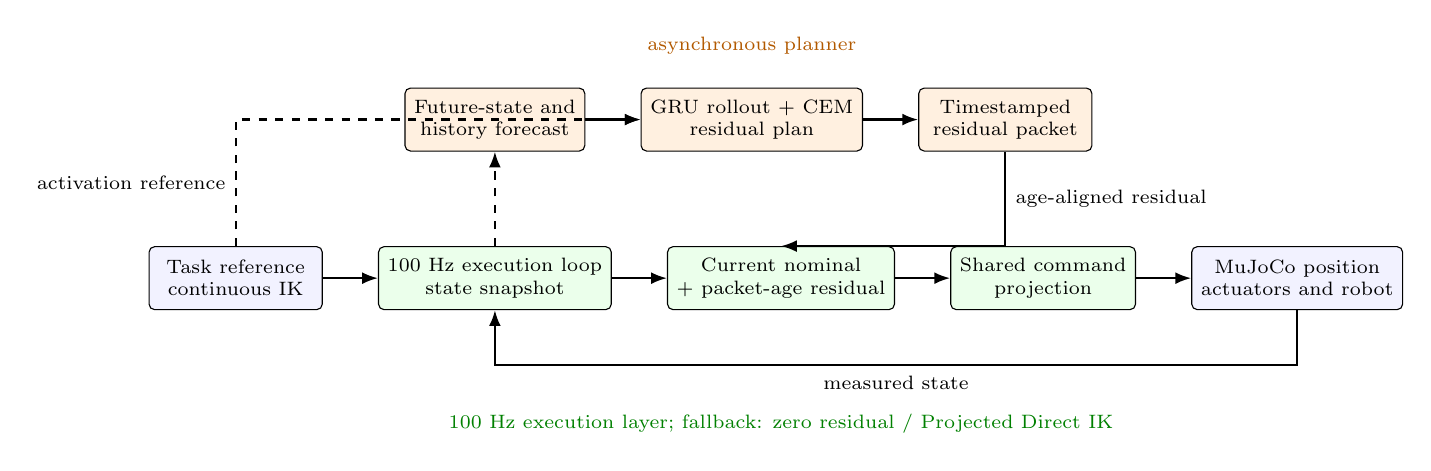
\begin{tikzpicture}[
  font=\scriptsize,
  box/.style={draw, rounded corners=2pt, align=center, minimum height=8mm, minimum width=22mm, fill=blue!5},
  fast/.style={box, fill=green!8},
  slow/.style={box, fill=orange!12},
  arrow/.style={-{Latex[length=2mm]}, thick},
  dashedarrow/.style={-{Latex[length=2mm]}, thick, dashed}
]
  \node[box] (ref) {Task reference\\continuous IK};
  \node[fast, right=7mm of ref] (loop) {100 Hz execution loop\\state snapshot};
  \node[slow, above=12mm of loop] (forecast) {Future-state and\\history forecast};
  \node[slow, right=7mm of forecast] (planner) {GRU rollout + CEM\\residual plan};
  \node[slow, right=7mm of planner] (packet) {Timestamped\\residual packet};
  \node[fast, right=7mm of loop] (anchor) {Current nominal\\+ packet-age residual};
  \node[fast, right=7mm of anchor] (project) {Shared command\\projection};
  \node[box, right=7mm of project] (plant) {MuJoCo position\\actuators and robot};

  \draw[arrow] (ref) -- (loop);
  \draw[arrow] (loop) -- (anchor);
  \draw[arrow] (anchor) -- (project);
  \draw[arrow] (project) -- (plant);
  \draw[arrow] (plant.south) |- ++(0,-7mm) -| node[pos=.25, below] {measured state} (loop.south);
  \draw[dashedarrow] (loop) -- (forecast);
  \draw[arrow] (forecast) -- (planner);
  \draw[arrow] (planner) -- (packet);
  \draw[arrow] (packet) |- node[pos=.25, right] {age-aligned residual} (anchor.north);
  \draw[dashedarrow] (ref.north) |- node[pos=.25, left] {activation reference} (planner.west);

  \node[above=3mm of planner, text=orange!70!black] {asynchronous planner};
  \node[below=12mm of anchor, align=center, text=green!50!black] {100 Hz execution layer; fallback: zero residual / Projected Direct IK};
\end{tikzpicture}

  \caption{Activation-aligned learned residual CEM-MPC. The asynchronous planner forecasts an activation state and publishes a timestamped residual packet. The 100~Hz layer rebuilds the current nominal, applies the age-aligned correction, and uses the same physical projection as the planner.}
  \label{fig:system}
\end{figure*}

\subsection{Future Anchor and Timestamped Packet}
At launch step $t_l$, the planner forecasts the commands expected while it runs and anchors the optimization at
\begin{equation}
 (\hat{\bm x}_{t_a},\hat{\mathcal H}_{t_a})=\hat F_\theta^{(D)}
 (\mathcal H_{t_l},\bm u^{\mathrm{active}}_{t_l:t_a-1}),
 \qquad t_a=t_l+D.
\end{equation}
Here $\mathcal H_t=[\bm z_{t-L+1},\ldots,\bm z_t]$ is the aligned $L=16$ token buffer. CEM rollouts begin from $\hat{\mathcal H}_{t_a}$, not merely $\hat{\bm x}_{t_a}$. The reference window begins at the activation anchor: $\bm q_k^d=\bm q_{t_a+k+1}^{\rm IK}$, and candidate command $\bm q_k^{\rm ref}$ produces $\hat{\bm x}_{k+1}$ aligned with that target. A completed solution is published with launch, publication, and activation timestamps, a residual sequence, and its predicted states. Packets published after the activation guard deadline are discarded.

At execution step $t$, packet age is $a=t-t_a$. If $0\leq a<H$, the fast loop retrieves $(\bm r_a,\hat{\bm x}_a)$ and computes
\begin{equation}
 \delta\bm r_t=\operatorname{clip}
 \left(K_q(\hat{\bm q}_a-\bm q_t)+K_{\dot q}(\hat{\dot{\bm q}}_a-\dot{\bm q}_t),
 -\delta\bm r_{\max},\delta\bm r_{\max}\right).
\end{equation}
The requested correction is
\begin{equation}
 \bm c_t=\operatorname{clip}(\bm r_a+\delta\bm r_t,
 -\bm r_{\max}-\delta\bm r_{\max},
 \bm r_{\max}+\delta\bm r_{\max}).
\end{equation}
If no valid packet exists, $\bm c_t=\bm0$.

\subsection{Execution Projection and Projected Direct-IK Fallback}
The 100~Hz layer rebuilds the current clipped IK nominal and applies the actual implementation rule
\begin{equation}
 \bm q_t^{\mathrm{cmd}}=
 \Pi_{v,a,\mathcal Q}(\bar{\bm q}^{\mathrm{IK}}_t+\bm c_t;
 \bm q_{t-1}^{\mathrm{cmd}},\dot{\bm q}_{t-1}^{\mathrm{cmd}}),
 \label{eq:execution}
\end{equation}
Zero correction therefore requests a projected Direct-IK nominal rather than bypassing command-rate limits. Zero and nonzero corrections both obey acceleration, velocity, braking, and joint-range limits. The executed residual is
\begin{equation}
 \bm r_t^{\mathrm{exec}}=\bm q_t^{\mathrm{cmd}}-\bar{\bm q}^{\mathrm{IK}}_t,
\end{equation}
which can differ from $\bm c_t$. We therefore measure projection activation; safety-projection offset RMS/P95/max; planner-requested versus executed residual and joint-reference discrepancy; residual/feedback saturation; and joint, velocity, and acceleration violations.

Virtual delay-aware MPC is a deterministic fixed-delay emulator launched at a prescribed interval. Wall-clock threaded MuJoCo execution instead uses a CUDA worker that consumes the latest snapshot after each solve; its update rate is set by measured wall-clock execution. Only the latter is treated as the final soft-real-time system.

\section{Experiments}
\label{sec:protocol}
One GRU checkpoint, normalizer, CEM budget, cost, constraints, anticipation delay, and feedback setting are selected on a separate calibration trajectory and then frozen. Tests use circle, figure-eight, fast ellipse, and rounded-square references. The square is smoothed to avoid attributing reference discontinuities to controller delay. Experiments use an NVIDIA RTX~4060 Laptop GPU with CUDA~13.0, PyTorch~2.11.0, MuJoCo~3.8.1, and Python~3.10.20; the manifest fixes the model, normalizer, XML, references, and clean commit.

The main evaluation separates deterministic IK baselines from stochastic MPC methods:
\begin{enumerate}
 \item \textbf{Raw Direct IK}: the unprojected nominal reference;
 \item \textbf{Projected Direct IK}: the practical nominal baseline using the shared physical projector;
 \item \textbf{Preview IK}: one preview selected on an independent calibration reference and frozen across test trajectories;
 \item \textbf{Ideal zero-delay logical MPC}: the solution is applied without advancing simulated time, providing a logical residual-MPC upper bound rather than a real-time controller;
 \item \textbf{Naive delayed/cached MPC}: a launch-state plan is applied after delay without current-nominal reconciliation;
 \item \textbf{Virtual delay-aware MPC}: deterministic fixed-delay validation of anchoring and reanchoring; and
 \item \textbf{Threaded asynchronous MPC}: the measured dual-thread implementation.
\end{enumerate}
Each deterministic IK method is run once under the fixed initial condition. MPC methods use five paired CEM seeds. The pre-specified primary endpoint is the trajectory--seed paired difference in full-trajectory TCP position RMSE between FullVirtual and NaiveDelayed. Comparisons with Projected Direct IK are secondary endpoints. Bootstrap resampling uses trajectory--seed cases, never individual 10~ms ticks, with 10,000 resamples. We report per-trajectory, aggregate, and worst-seed results with 95\% paired-bootstrap confidence intervals. The representative plot uses the nominal circle ThreadedASAP seed whose TCP RMSE is closest to the five-seed median. The three component-ablation contrasts are not additive independent effects.

CEM solve latency covers only \texttt{controller.plan()}. Planner end-to-end latency runs from snapshot launch to packet publication and determines whether a packet is late. We separately report solve and end-to-end p50/p95/p99/max, actual planner update rate, late and expired packets, fallback duty cycle, fast-loop compute time, control-period p95/p99, wake-up jitter, deadline misses, and the worst seed.

\begin{table*}[!t]
\caption{Nominal tracking and control-quality means under the frozen configuration. IK rows average four deterministic trajectories; MPC rows average 20 trajectory--seed cases. Paired confidence intervals for the pre-specified contrasts are reported in the text.}
\label{tab:tracking}
\centering
\footnotesize
\resizebox{\textwidth}{!}{%
\begin{tabular}{lcccccc}
\toprule
Method & TCP RMSE & TCP P95 & Orient. RMSE & Joint RMSE & Cmd. accel. RMS & Torque RMS \\
 & (mm)$\downarrow$ & (mm)$\downarrow$ & (deg)$\downarrow$ & (rad)$\downarrow$ & (rad/s$^2$) & (Nm) \\
\midrule
Raw Direct IK & 39.26 & 89.63 & 2.01 & 0.0148 & 0.58 & 5.60 \\
Projected Direct IK & 39.26 & 89.63 & 2.01 & 0.0148 & 0.58 & 5.60 \\
Preview IK & 32.64 & 74.75 & 2.04 & 0.0120 & 0.58 & 5.60 \\
Ideal zero-delay logical MPC & 28.15 & 57.24 & 1.42 & 0.0117 & 6.51 & 20.96 \\
Naive delayed/cached MPC & 67.93 & 140.20 & 11.65 & 0.0901 & 7.89 & 4.47 \\
Virtual delay-aware MPC & 28.37 & 58.70 & 1.46 & 0.0117 & 6.69 & 17.17 \\
Threaded asynchronous MPC & 28.43 & 59.07 & 1.44 & 0.0116 & 6.74 & 16.25 \\
\bottomrule
\end{tabular}}
\end{table*}

\begin{table*}[!t]
\caption{Nominal ThreadedASAP deployment timing. Solve and E2E values are milliseconds. ``Late'' is late packets divided by planner solves; deadline misses are fast-loop ticks. Projection offset is in mrad.}
\label{tab:timing}
\centering
\footnotesize
\resizebox{\textwidth}{!}{%
\begin{tabular}{cccccccccc}
\toprule
Solve p50/p95/p99/max & E2E p50/p95/p99/max & Planner & Fast loop & Period & Wake lateness & Late packets & Fallback & Deadline misses & Projection \\
 & & Hz & p99 & p95/p99 & p95 & & duty & & active / offset p95 \\
\midrule
36.57/38.27/41.96/171.30 & 44.92/49.04/51.94/180.48 & 25.30 & 1.089 & 10.093/10.158 & 0.266 & 34 / 0.388\% & 0.355\% & 12 / 34,640 (0.0346\%) & 85.48\% / 36.47 \\
\bottomrule
\end{tabular}}
\end{table*}

\section{Results}
\label{sec:results}

\subsection{Stale-Plan Degradation and Recovery}
The primary comparison is the paired full-trajectory TCP position RMSE difference between FullVirtual and NaiveDelayed. Projected Direct IK is the key practical secondary baseline, while Ideal zero-delay logical MPC is a non-deployable logical upper bound. In addition to raw errors, define
\begin{equation}
 R_{\mathrm{latency}}=
 \frac{E_{\mathrm{naive}}-E_{\mathrm{ASAP}}}
 {E_{\mathrm{naive}}-E_{\mathrm{zero-delay}}}.
\end{equation}
FullVirtual averaged 28.37~mm TCP RMSE, close to the 28.15~mm logical zero-delay result, whereas NaiveDelayed averaged 67.93~mm. The paired FullVirtual--NaiveDelayed difference was $-39.55$~mm (95\% CI $-42.10$ to $-36.87$~mm), a mean reduction of 58.1\%. The same direction held on circle ($-40.10$~mm), fast ellipse ($-40.19$~mm), figure-eight ($-37.18$~mm), and rounded square ($-40.75$~mm). Orientation RMSE also fell by 0.178~rad (95\% CI $-0.188$ to $-0.167$~rad). The recovery ratio was 1.004 (95\% CI 0.958--1.059) over the 20 paired cases; it is reported only because every paired denominator was positive.

\begin{figure}[!t]
 \centering
 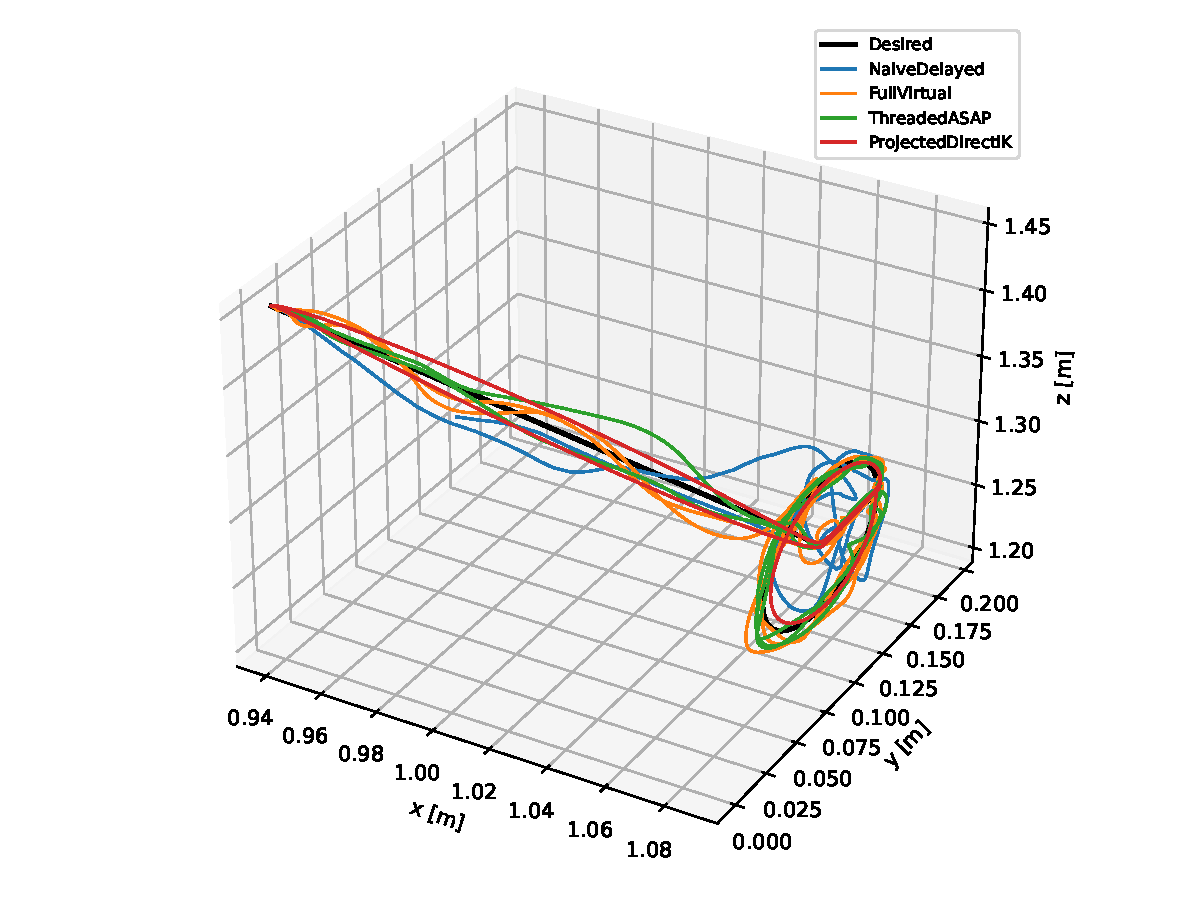
\includegraphics[width=\columnwidth]{figures/representative_tracking.pdf}
 \caption{Pre-specified nominal circle representative: the ThreadedASAP seed closest to the five-seed median. Desired and actual TCP paths use the common reference and constraints.}
\label{fig:tracking}
\end{figure}

\subsection{Threaded Deployment and Robustness}
Under nominal conditions, ThreadedASAP averaged 28.43~mm TCP RMSE and differed from FullVirtual by +0.054~mm (95\% CI $-1.094$ to +1.303~mm). It reduced nominal TCP RMSE by 10.84~mm relative to Projected Direct IK (95\% CI $-11.80$ to $-9.55$~mm) and by 4.21~mm relative to Preview IK (95\% CI $-5.11$ to $-2.98$~mm). The advantage over Projected IK persisted under payload, actuator-gain, force-pulse, and observation-noise perturbations. Nominal agreement did not imply equality under every perturbation: actuator-gain disturbance increased ThreadedASAP RMSE by 3.20~mm relative to FullVirtual (95\% CI 2.40--4.05~mm).

\subsection{Timing, Control Quality, and Packet Behavior}
CEM solve p50/p95 was 36.57/38.27~ms and snapshot-to-publication p50/p95 was 44.92/49.04~ms, both slower than one command tick. The fast loop nevertheless used 0.470/0.887~ms at p50/p95 and maintained control-period p95/p99 of 10.093/10.158~ms. We observed 12 deadline misses in 34,640 ticks, a 0.388\% late-packet rate, one expiration, and 0.355\% fallback duty. The 132.45~ms worst period rules out a hard-real-time claim.

\begin{figure}[!t]
 \centering
 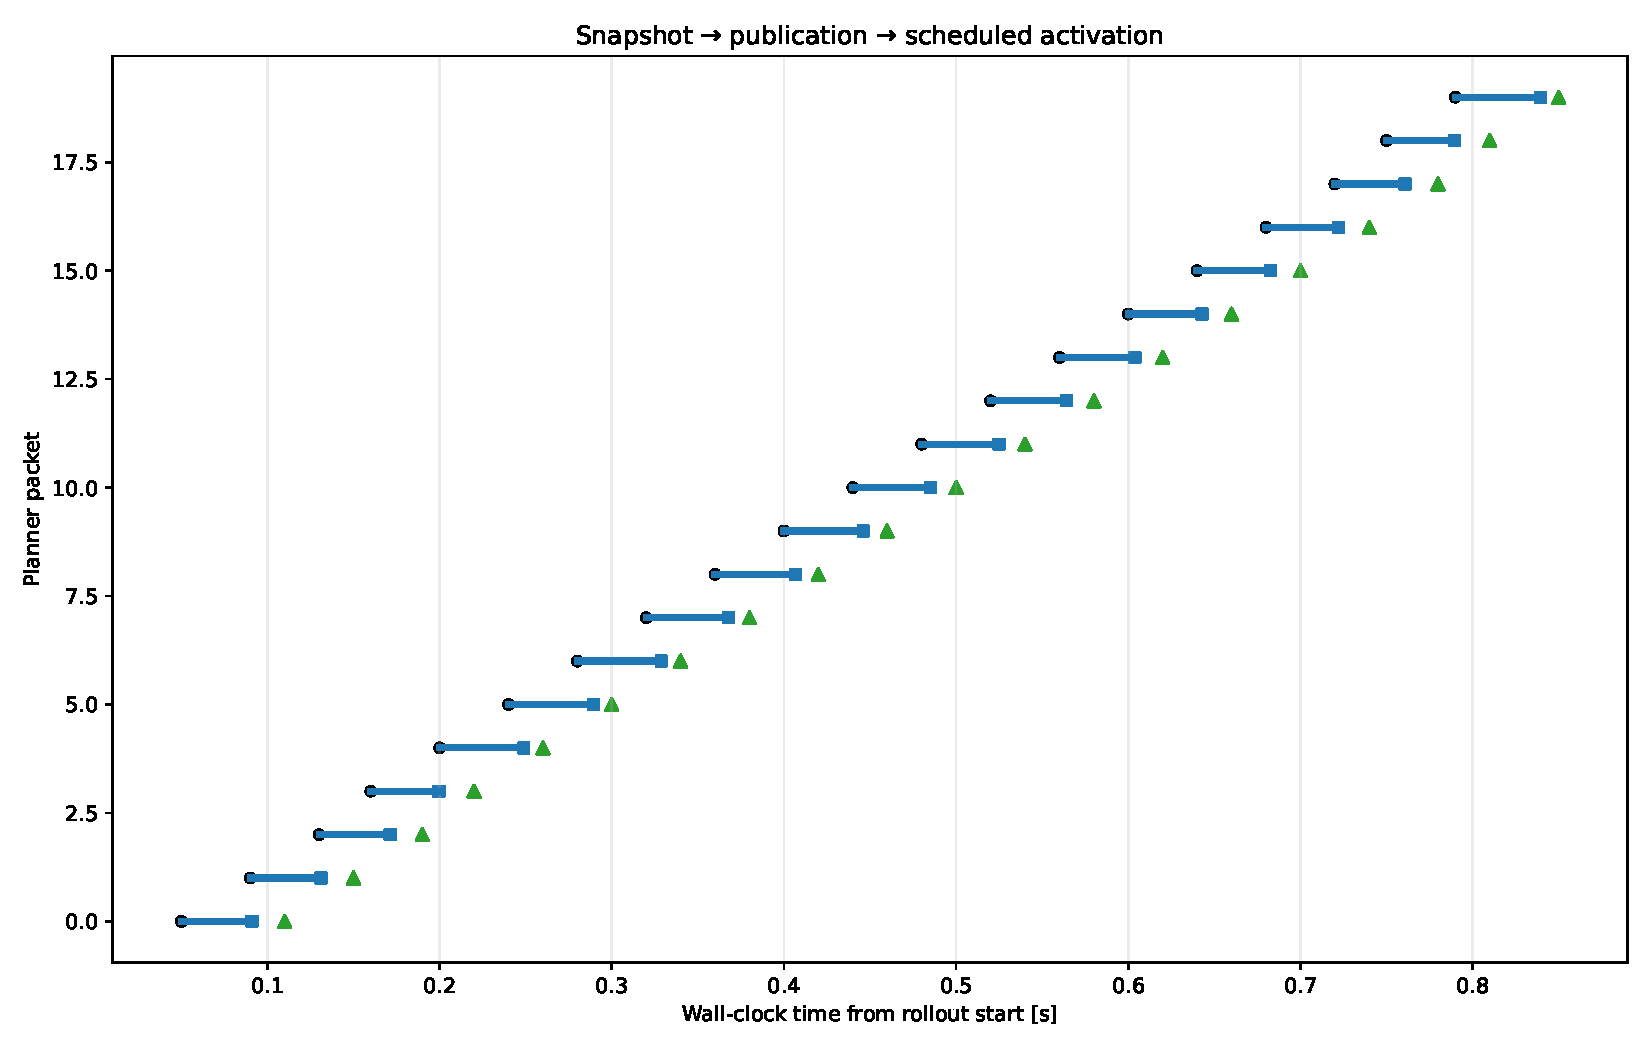
\includegraphics[width=\columnwidth]{figures/planner_timeline.pdf}
 \caption{Planner end-to-end and execution-layer timing.}
 \label{fig:timing}
\end{figure}

\subsection{Controlled Mechanism-Isolation Ablations}
\begin{table}[!t]
\caption{Matched removal contrasts against FullVirtual under the frozen virtual fixed-delay configuration. Positive values indicate worse TCP RMSE after removal.}
\label{tab:ablation}
\centering
\footnotesize
\resizebox{\columnwidth}{!}{%
\begin{tabular}{lcc}
\toprule
Removal & $\Delta$ TCP RMSE & 95\% CI \\
\midrule
No future alignment & +2.82 mm & [1.27, 4.39] mm \\
No re-anchor & +654.60 mm & [528.68, 778.68] mm \\
No feedback & $-0.95$ mm & [$-2.25$, 0.28] mm \\
\bottomrule
\end{tabular}}
\end{table}
All 20 FullVirtual anchors were rerun under the same frozen commit and schema as the 60 removal runs. Removing future alignment increased TCP RMSE by 2.82~mm (95\% CI 1.27--4.39~mm), while removing execution-time reanchoring increased it by 654.60~mm (528.68--778.68~mm). Removing fast feedback changed RMSE by $-0.95$~mm ($-2.25$--0.28~mm), so this experiment does not establish an independent tracking benefit for feedback. The contrasts share references, constraints, CEM budgets, and paired seeds, but are neither independent nor additive.

\subsection{Planner-Delay Sweep}
Virtual experiments impose $D\in\{2,4,6,8\}$ steps, corresponding to 20, 40, 60, and 80~ms. They compare naive delayed execution, future anchoring only, anchoring plus nominal/residual reanchoring, and the full method with fast feedback.
The results do not form a monotone component ladder. Anchor-only TCP RMSE was 30.9 and 29.6~mm at $D=2,4$, but rose to 831.4 and 941.2~mm at $D=6,8$. The reanchored variant remained between 29.1 and 32.4~mm. Thus reanchoring is necessary for future alignment to remain stable through an absolute-position command interface at larger delays; fast feedback is treated as an auxiliary correction.
\begin{figure}[!t]
 \centering
 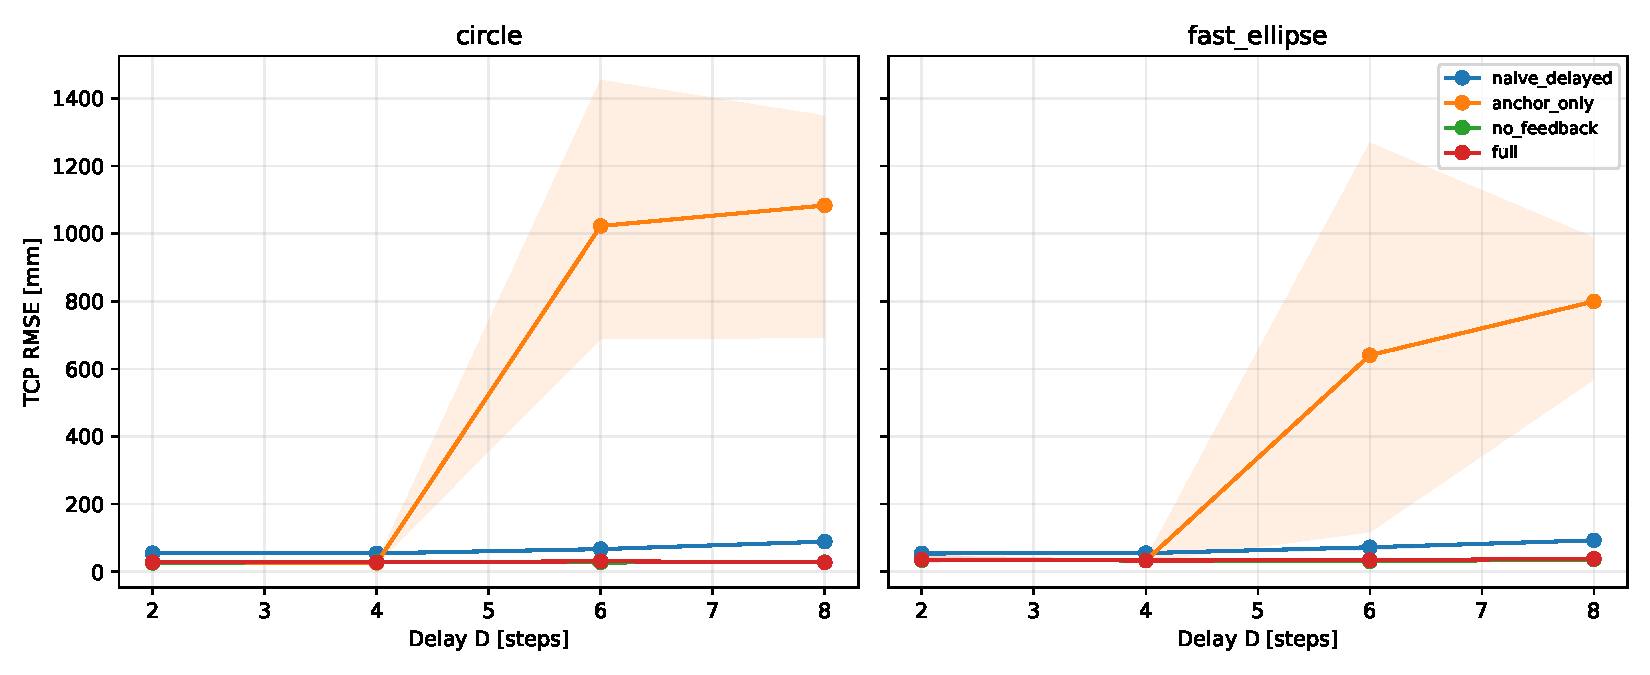
\includegraphics[width=\columnwidth]{figures/delay_sweep.pdf}
 \caption{Sensitivity to imposed planner delay under deterministic virtual scheduling.}
 \label{fig:delay-sweep}
\end{figure}

\subsection{Task-Space Final-Pool Cost Ablation}
We isolate the effect of final-pool task-space reranking on circle and figure-eight trajectories with three paired CEM seeds. Joint-only and task-space variants first share fixed $D=6$ virtual delay. They are then run as wall-clock threaded MuJoCo deployments using their separately calibrated delays, so the deployment comparison includes reranking cost. In threaded deployment, task-space reranking reduced TCP RMSE by 3.05~mm (95\% CI 0.96--4.32~mm) while increasing E2E p95 by 6.82~ms. We therefore report an accuracy--latency trade-off, not an unqualified improvement.

\begin{figure}[!t]
 \centering
 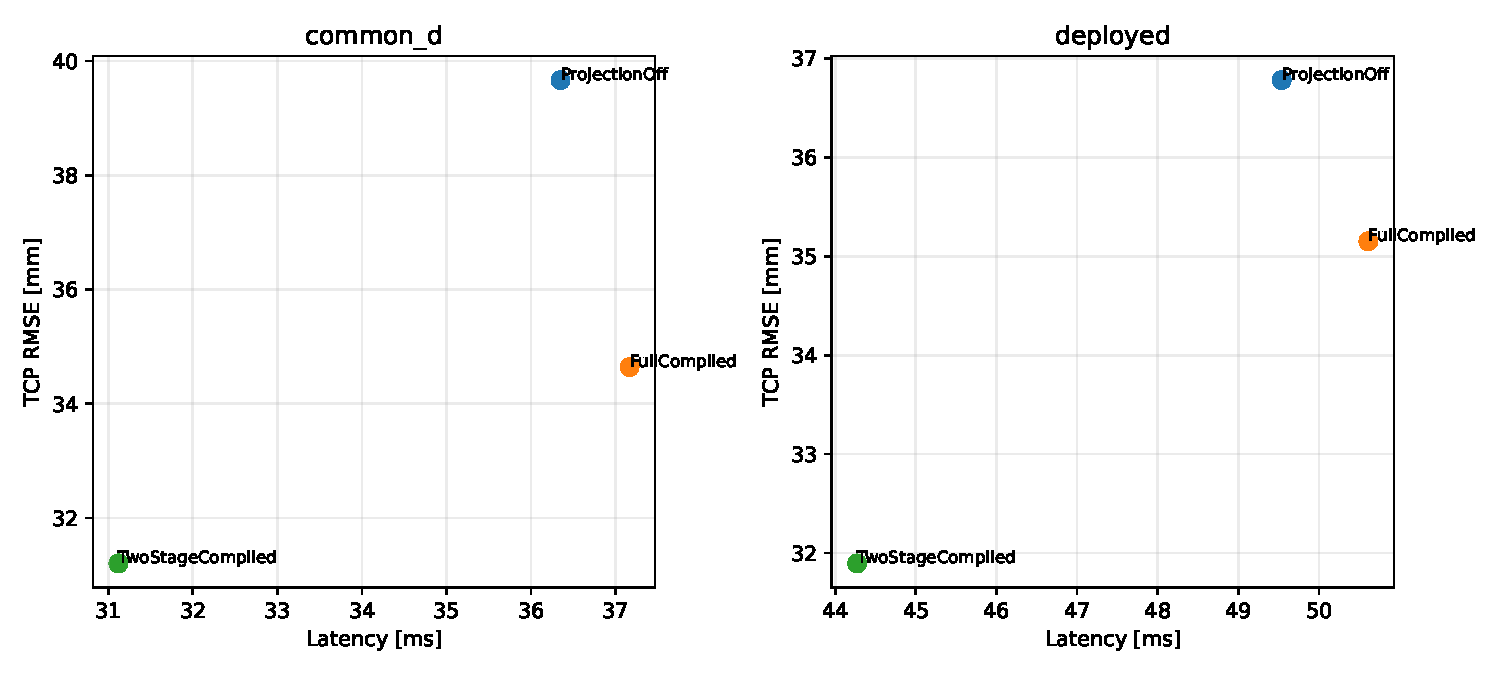
\includegraphics[width=\columnwidth]{figures/projection_tradeoff.pdf}
 \caption{Projection-choice diagnostic. Two-stage compiled projection was non-inferior to full compiled projection under the pre-specified 5\% TCP-RMSE margin while reducing the computation--consistency burden.}
 \label{fig:projection-tradeoff}
\end{figure}

\section{Results and Discussion}
\label{sec:discussion}
The primary mechanism claim comes from the paired FullVirtual--NaiveDelayed comparison. As a secondary deployment result, ThreadedASAP also outperformed Projected Direct IK under nominal conditions and under every tested perturbation category. It outperformed Preview IK overall and under nominal, payload, actuator-gain, and force-pulse conditions; under observation noise, the mean difference was +0.95~mm with a 95\% CI of $-0.49$--2.56~mm and was not significant. Any interpretation must account for the gap between the planner-requested command in~\eqref{eq:planner-request} and the execution-projected command in~\eqref{eq:execution}.

The scope is limited to an ABB IRB~2400 MuJoCo model, one frozen learned model and compute platform, and Python soft-real-time threading. No physical-robot or hard-real-time claim is made, and the method has no theoretical stability guarantee. Future-state alignment and execution-time reanchoring constitute the supported mechanism claim. Fast feedback is an auxiliary state correction; task-space reranking trades accuracy for latency; and two-stage projection manages computation--consistency trade-offs. Projection was active on 85.48\% of nominal threaded ticks, so execution projection materially shapes the dispatched commands.

\section{Conclusion}
Future activation alignment and execution-time residual reanchoring recovered the stale-plan loss of a learned residual CEM planner: FullVirtual reduced TCP RMSE by 39.55~mm, or 58.1\%, relative to NaiveDelayed. Under nominal conditions, ThreadedASAP matched FullVirtual within 0.054~mm (95\% CI $-1.094$--1.303~mm) while using a 25.30~Hz planner behind the 100~Hz execution layer. Its 44.92/49.04~ms E2E p50/p95 confirms that planning is slower than the command period. These conclusions are limited to the ABB IRB~2400 MuJoCo model and Python soft-real-time deployment; they do not establish an independent feedback gain, hard-real-time behavior, or unrestricted model generalization.

\bibliographystyle{IEEEtran}
\bibliography{references}
\end{document}
